
\begin{figure} \begin{center}
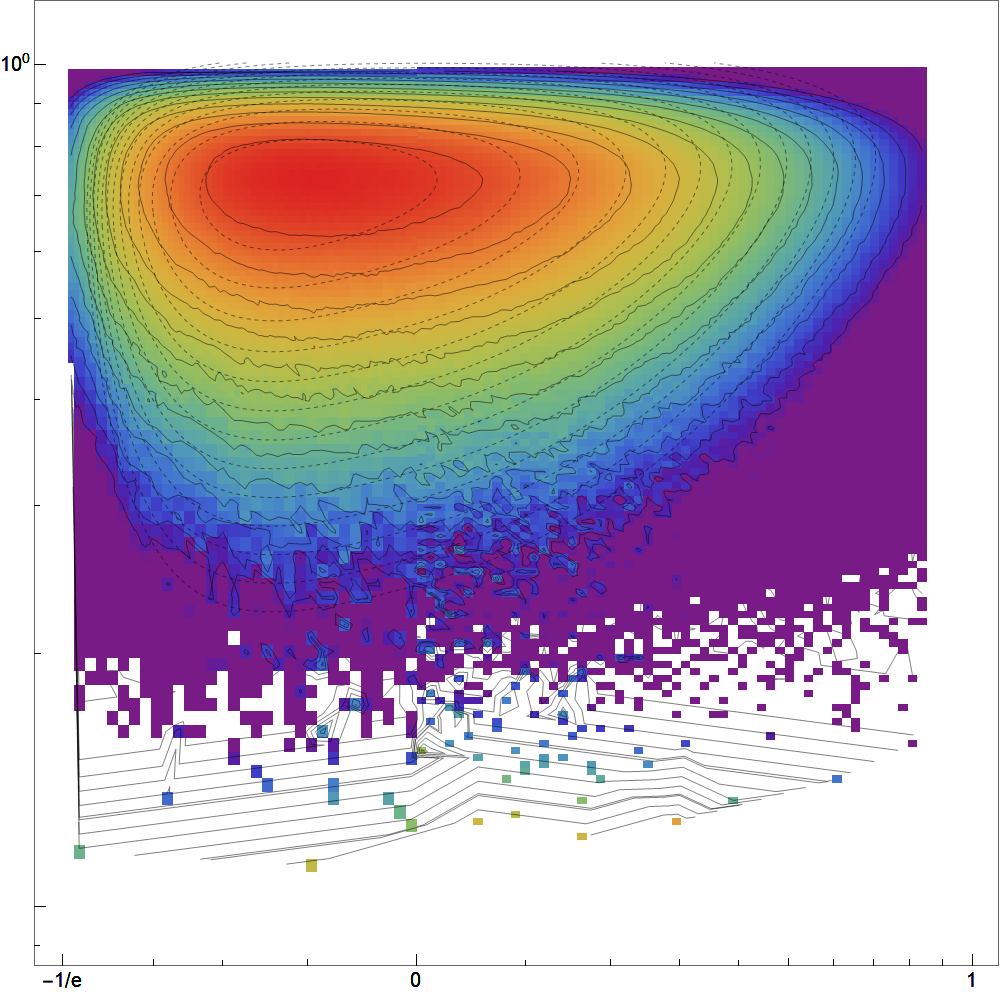
\includegraphics[width=0.32\textwidth]{figs/mach5_contours_comparison_V_MCMC.png}
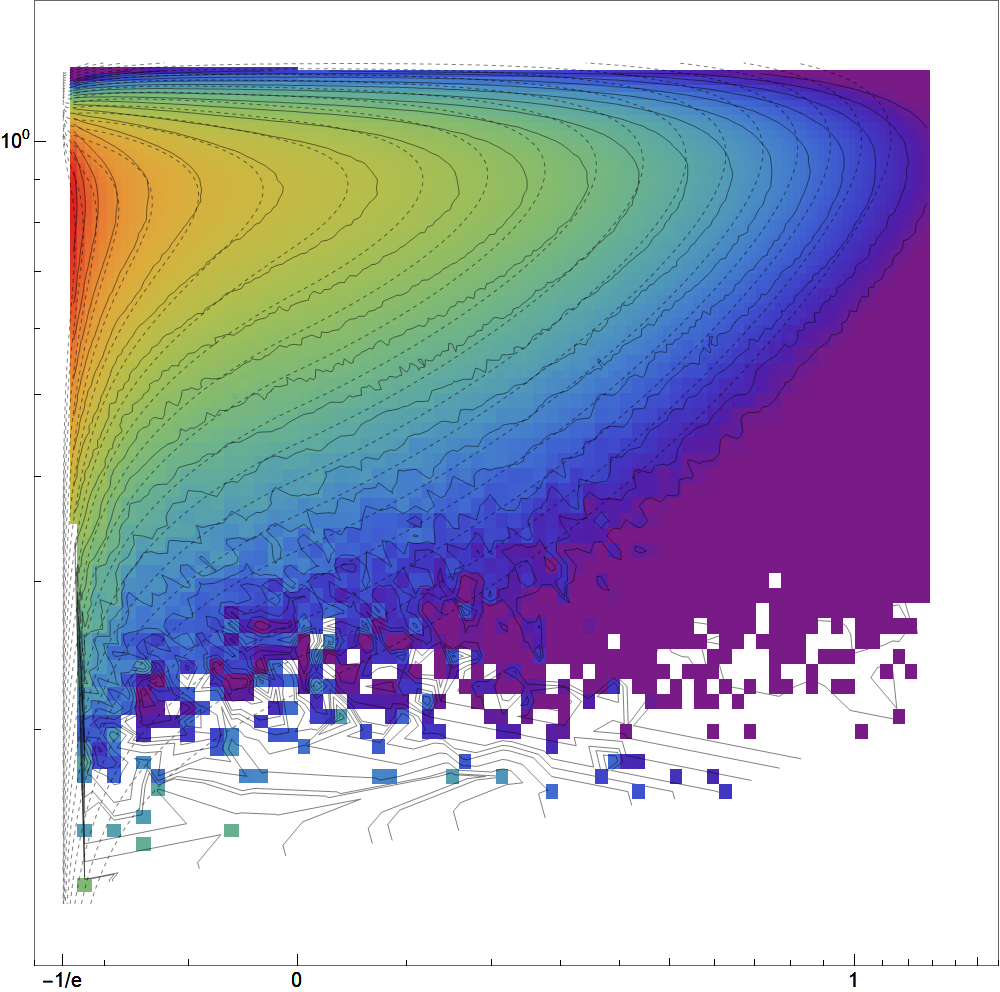
\includegraphics[width=0.32\textwidth]{figs/mach10_contours_comparison_V_MCMC.png}
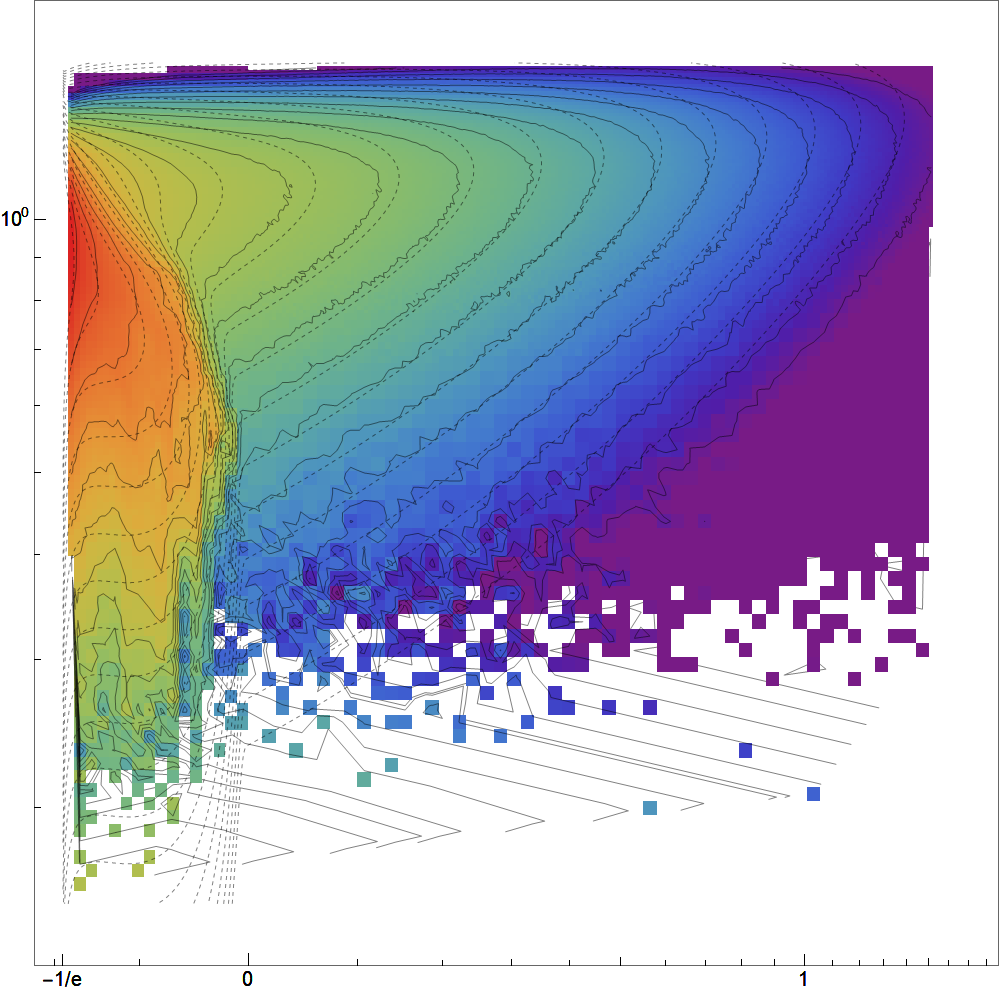
\includegraphics[width=0.32\textwidth]{figs/mach20_contours_comparison_V_MCMC.png}
\caption[ ]{The joint distribution between thermal energy, $E_T$ (horizontal), and kinetic
energy $E_K$ (vertical). Color shows the PDF computed from low resolution simulations, and ranges between 0 (purple) and 1
(red).  The thermal energy develops a low $E_T$ wall as well as a high $E_T$
wing as the Mach number increases.  Dashed lines are our analytic estimate,
which is good but has differences that are likely due to resolution. }
\label{fig.energy} \end{center} \end{figure}
